\documentclass{article}
\usepackage{v-test-paper}
\title{\textsc{Error Analysis}}
\date{February 22, 2024}

\newcommand{\itemstared}{\refstepcounter{enumi}\item[$^\star$\theenumi.]}
\usetikzlibrary{matrix,  positioning, patterns, backgrounds}
\renewcommand{\ans}{\quad}


\tikzstyle{root} = [rectangle, rounded corners, 
minimum width=3cm, 
minimum height=0.7cm,
text centered, 
draw, 
font=\scshape,
]
\tikzstyle{child} = [rectangle, rounded corners, 
inner sep=2mm,
text centered, 
draw, 
font=\itshape,
text width=3.25cm,
]

\tikzstyle{child-branch} = [
    rectangle, 
    rounded corners, 
    inner sep=2mm,
    text centered, 
    draw, 
    font=\itshape,
    text width=2.5cm,
    level distance=5mm,
]



\tikzstyle{arrow} = [thick,->,>=latex]


\begin{document}
\maketitle
\begin{center}
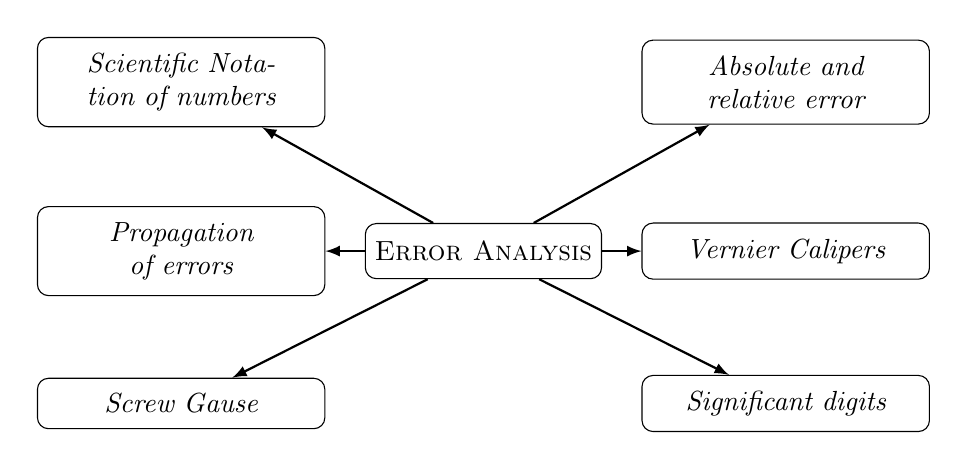
\begin{tikzpicture}[node distance=2cm]

\matrix [column sep=5mm,row sep=10mm]
{
\node (child-left)[child] {Scientific Notation of numbers}; & &
\node (child-right)[child] {Absolute and relative error}; \\
\node (child-left-b)[child] {Propagation of errors}; & 
\node (root) [root] {Error Analysis};&
\node (child-right-b)[child] {Vernier Calipers}; \\
\node (child-left-bb)[child] {Screw Gause}; & &
\node (child-right-bb)[child]{Significant digits};\\
};

\draw [arrow] (root) -- (child-left);
\draw [arrow] (root) -- (child-right);
\draw [arrow] (root) --(child-left-b);
\draw [arrow] (root) -- (child-right-b);
\draw [arrow] (root) -- (child-right-bb);
\draw [arrow] (root)--(child-left-bb);
\end{tikzpicture}
\end{center}

\centering\textsc{Rules for significant figures}
\begin{enumerate}
    \item All non-zero digits are significant.
    \item Zeros between non-zero digits are significant.
    \item Leading zeros are not significant.
    \item Trailing zeros in a number without a decimal point are not significant.
    \item Trailing zeros in a number with a decimal point are significant.
    \item The power of 10 in a number in scientific notation is not significant.
    \item If a measurement is less than 1, then all zeros occurring to the left of the last non-zero digit are not significant.
    \item Change in units of measurement does not affect the number of significant figures.
    \item Exact measurements have an infinite number of significant figures.
\end{enumerate}

\vspace*{8mm}

\begin{center}
    \textsc{Problems}
\end{center}
\begin{enumerate}
    \item The mass and density of a solid sphere are measured to be $\left(12.4\pm 0.1\right)\kg$ and $\left(4.6\pm 0.2\right)\kg/\m^3$ respectively. The volume of the sphere with error limits is
    \begin{tasks}(2)
        \task $\left(2.7\pm 0.14\right)\m^3$\ans
        \task $\left(2.7\pm 0.3\right)\m^3$
        \task $\left(2.7\pm 0.4\right)\m^3$
        \task $\left(2.7\pm 0.5\right)\m^3$
    \end{tasks}

    \item Maximum percentage error in determination of time period of a pendulum \[ T=2\pi\sqrt{\dfrac{l}{g}} \] where, $l$ and $g$ are measured with $\pm 1\%$ ans $\pm 2\%$ error respectively, is
    \begin{tasks}(2)
        \task $\pm 1\%$
        \task $\pm 1.5\%$\ans
        \task $\pm 2\%$
        \task $\pm 2.5\%$
    \end{tasks}

    \item Round off $231.45$ to two significant digits.
    \begin{tasks}(4)
        \task $230$\ans
        \task $231$
        \task $231.5$
        \task $231.45$
    \end{tasks}

    \item Calculate equivalent resistance of two resistors $R_1$ and $R_2$ connected in parallel with $R_1=\left(6\pm 0.2\right)\Ohm$ and $R_2=\left(3\pm 0.1\right)\Ohm$. 
    \begin{tasks}(2)
        \task $\left(2\pm 0.01\right)\Ohm$
        \task $\left(2\pm 0.07\right)\Ohm$\ans
        \task $\left(2\pm 0.20\right)\Ohm$
        \task $\left(2\pm 0.50\right)\Ohm$
    \end{tasks}

    \item The least count of the main scale of a screw gauge is $1 \mm$. The minimum number of divisions on its circular scale required to measure $5 \upmu\!\m$ diameter of a wire is
    \begin{tasks}(4)
        \task $50$
        \task $100$
        \task $200$\ans
        \task $500$
    \end{tasks}

    \item A student uses a simple pendulum of exactly $1\m$ length to determine $g$, the acceleration due to gravity. He uses a stop watch with the least count of $1 \s$ for this and records $40 \s$ for $20$ oscillations. For this observation, which of the following statement(s) is/are true?
    \begin{tasks}
        \task Error $\Delta T$ in measuring $T$, the time period is $0.05 \s$\ans
        \task Error $\Delta T$ in measuring $T$, the time period is $1 \s$
        \task Percentage error in determination of $g$ is $5\%$\ans
        \task Percentage error in determination of $g$ is $2.5\%$
    \end{tasks}

    \item The pitch of a screw gauge is $1 \mm$ and there are $100$ divisions on the circular scale. In measuring the diameter of a sphere there are $6$ divisions on the linear scale and $40$ divisions on circular scale coincide with the reference line. Find the diameter of the sphere.
    \begin{tasks}(2)
        \task $6.4 \mm$\ans
        \task $4.6 \mm$
        \task $6.4 \cm$
        \task $4.6 \cm$
    \end{tasks}

    \item The smallest division on main scale of a vernier calipers is $1 \mm$ and $10$ vernier divisions coincide with $9$ main scale divisions. What would be the least count of the vernier calipers?
    \begin{tasks}(2)
        \task $0.01 \cm$\ans
        \task $0.02 \cm$
        \task $0.03 \cm$
        \task $0.04 \cm$
    \end{tasks}

    \item The smallest division on main scale of a vernier calipers is $1 \mm$ and $10$ vernier divisions coincide with $9$ main scale divisions. While measuring the length of a line, the zero mark of the vernier scale lies between $10.2 \cm$ and $10.3 \cm$ and the third division of vernier scale coincides with a main scale division. What would be the length of the line?
    \begin{tasks}(2)
        \task $10.01 \cm$
        \task $10.23 \cm$\ans
        \task $10.03 \cm$
        \task $10.10 \cm$
    \end{tasks}

    \item In a vernier calipers, $N$ divisions of the main scale coincide with $N + m$ divisions of the vernier scale. What is the value of $m$ for which the instrument has minimum least count.
    \begin{tasks}(4)
        \task $4$
        \task $3$
        \task $2$
        \task $1$\ans
    \end{tasks}


    

    


\end{enumerate}


\pagebreak

\begin{center}
\texttt{Answer Key}
\begin{multicols}{5}
\begin{enumerate}
\item (b)
\item (b)
\item (a)
\item (b)
\item (d)
\item (b)
\item (c)
\item (a), (b)
\item (c)
\item (a), (b), (c), (d)
\end{enumerate}
\end{multicols}
\end{center}






\end{document}